% ===========================================================================
% 第四章 实验与分析
% ===========================================================================
\chapter{实验与分析}

本章通过实验验证\ScaffoldChunGS 系统的功能完整性与性能指标。实验分为四部分：（1）压缩效果定量分析；（2）分块内存管理行为分析；（3）关键参数的消融实验；（4）KITTI数据集实验。

\section{实验环境与配置}

\subsection{硬件与软件环境}

\begin{table}[htbp]
\centering
\caption{实验环境配置}
\label{tab:env}
\begin{tabular}{ll}
\toprule
\textbf{项目} & \textbf{配置} \\
\midrule
GPU & NVIDIA Jetson Orin Nano (8 GB, sm\_87) \\
CPU & 6-core ARM Cortex-A78AE @ 1.5 GHz \\
CUDA & 11.4 (JetPack 5.1.3) \\
LibTorch & 2.1.0 (aarch64, prebuilt) \\
OpenCV & 4.8.0 (with CUDA, JetPack) \\
Eigen3 & 3.4.0 \\
编译器 & GCC 9.5 + NVCC 11.4 \\
\bottomrule
\end{tabular}
\end{table}

\subsection{默认超参数设置}

除非特别说明，所有实验使用表\ref{tab:default_hp}中的默认超参数（与 \texttt{scaffold\_chunks.yaml} 一致）。

\begin{table}[htbp]
\centering
\caption{默认超参数}
\label{tab:default_hp}
\begin{tabular}{lrl}
\toprule
\textbf{参数} & \textbf{值} & \textbf{说明} \\
\midrule
$K$ (n\_offsets) & 5 & 每锚点子高斯数 \\
$D$ (feat\_dim) & 32 & 锚点特征维度 \\
$v_s$ (voxel\_size) & 0.01 m & 体素尺寸 \\
$S$ (chunk\_size) & 20.0 & 块边长（世界单位） \\
$M_{\max}$ & 120,000 & GPU锚点上限（8 GB Jetson） \\
$\lambda_{\text{SSIM}}$ & 0.2 & SSIM损失权重 \\
$\lambda_{\text{depth}}$ & 0.1 & 深度损失权重 \\
$\lambda_{\text{iso}}$ & 0.01 & 各向同性权重 \\
\text{update\_depth} & 3 & 层级生长深度 \\
\text{densify\_interval} & 100 & 稠密化间隔（迭代） \\
\bottomrule
\end{tabular}
\end{table}

\section{压缩效果分析}

\subsection{理论压缩比}

如表\ref{tab:compression_theory}所示，在标准配置下（$D=32$，$K=5$），\ScaffoldChunGS 的理论存储压缩比约为8.6倍。

\begin{table}[htbp]
\centering
\caption{理论存储压缩分析}
\label{tab:compression_theory}
\begin{tabular}{lrr}
\toprule
\textbf{项目} & \textbf{标准3DGS} & \textbf{Scaffold-ChunGS} \\
\midrule
参数/高斯 & 59 floats & -- \\
参数/锚点 & -- & $3+3K+6+4+1+D$ floats \\
Bytes/高斯 & $\sim$240 & $\sim$28（均摊，$K=5$） \\
MLP参数量 & 0 & $\sim$3$\times$(D$\times$D) $\approx$ 3K floats \\
\bottomrule
\end{tabular}
\end{table}

\subsection{不同$K$的压缩-质量权衡}

为确定最优的$K$（子高斯数/锚点），固定其他超参数（$D=32$，$v_s=0.01$），在XXX场景（场景名待填）上对比不同$K$值下的实际存储开销与渲染质量。

\begin{table}[htbp]
\centering
\caption{不同$K$值的压缩-质量对比（场景：KITTI/seq05，\#Gaussians $\approx$ 8.0$\times 10^5$）}
\label{tab:k_tradeoff}
\begin{tabular}{lrrrrrr}
\toprule
\textbf{$K$} & \textbf{压缩比} & \textbf{磁盘占用} & \textbf{PSNR} & \textbf{SSIM} & \textbf{LPIPS} & \textbf{训练时间} \\
 & \textbf{（理论）} & \textbf{（MB）} & \textbf{（dB）$\uparrow$} & $\uparrow$ & $\downarrow$ & \textbf{（min）} \\
\midrule
3  & 5.1$\times$ & XXX & XX.XX & X.XXX & X.XXX & XXX \\
5  & 8.6$\times$ & XXX & XX.XX & X.XXX & X.XXX & XXX \\
7  & 12.0$\times$ & XXX & XX.XX & X.XXX & X.XXX & XXX \\
10 & 17.1$\times$ & XXX & XX.XX & X.XXX & X.XXX & XXX \\
\bottomrule
\end{tabular}
\end{table}

实验预期：随$K$增大，理论压缩比线性提升，但渲染质量（PSNR/SSIM）可能逐步下降——每个锚点需表达更多子高斯，预测粒度变粗。最优$K$应选取质量-存储Pareto前沿上的转折点。

值得注意的是，Scaffold-GS\cite[Section~4.2, Fig.~9]{lu2024scaffoldgs}在静态场景重建中报告$K$值对最终激活高斯数影响不显著——模型通过opacity阈值$\tau_\alpha$自动过滤冗余高斯，激活数趋于收敛。然而，该结论在SLAM场景下未必成立：（1）SLAM为在线增量训练，锚点持续生长与淘汰，难以达到静态重建的收敛稳态；（2）视角稀疏且分布不均，部分锚点始终处于欠观测状态，自正则效率受限；（3）Jetson平台显存仅8 GB，$K$直接决定GPU端子高斯总数，即使冗余高斯最终被剪枝，训练过程中的峰值显存开销仍随$K$线性增长。因此，本实验将在SLAM条件下重新审视$K$的压缩-质量权衡。

\section{分块内存管理分析}

\subsection{LRU淘汰行为验证}

\subsubsection{实验场景设计}

为验证LRU淘汰机制的正确性，构建合成测试场景：将$100\,\text{m}\times 100\,\text{m}\times 60\,\text{m}$的空间区域划分为$5\times 5\times 3=75$个块，块边长$S=20$世界单位，块内锚点数量在4,000--18,000范围内均匀随机分布，场景总锚点数约$8.5\times 10^5$，远超GPU锚点上限$M_{\max}=300,000$。

相机以Zigzag轨迹遍历场景，水平视场角70°，垂直视场角50°，远裁剪面60 m，模拟车辆在KITTI场景中的运动模式。每帧仅加载可见块（与相机视锥重叠的块），超过$M_{\max}$时触发LRU淘汰。

\begin{table}[htbp]
\centering
\caption{LRU验证实验场景参数}
\label{tab:lru_setup}
\begin{tabular}{ll}
\toprule
\textbf{参数} & \textbf{值} \\
\midrule
块网格 & $5\times 5\times 3 = 75$ \\
场景范围 & $100\times 100\times 60$ m \\
块边长 $S$ & 20.0 世界单位 \\
锚点数/块 & 4,000--18,000（均匀随机） \\
场景总锚点数 & 850,792 \\
GPU锚点上限 $M_{\max}$ & 300,000 \\
滞后缓冲区 & 15,000（$M_{\max}$的5\%） \\
模拟帧数 & 200 \\
\bottomrule
\end{tabular}
\end{table}

\subsubsection{GPU锚点数量稳定性}

如图\ref{fig:lru_gpu_stability}所示，在200帧的模拟过程中，GPU常驻锚点数始终保持在$M_{\max}=300,000$以下（最大值299,935，最小值186,992），均值为276,382，标准差为25,194。0\%的帧超过$M_{\max}$，验证了LRU淘汰机制能有效维持GPU显存占用在预设上限之内。

值得注意的是，轨迹起始阶段锚点数从约187K逐步上升（相机刚进入场景，可见块数较少），约在第25帧后进入稳态波动，后续始终在250K--300K之间浮动，证明系统的稳态显存行为具有良好的自稳定特性。

\begin{figure}[htbp]
\centering
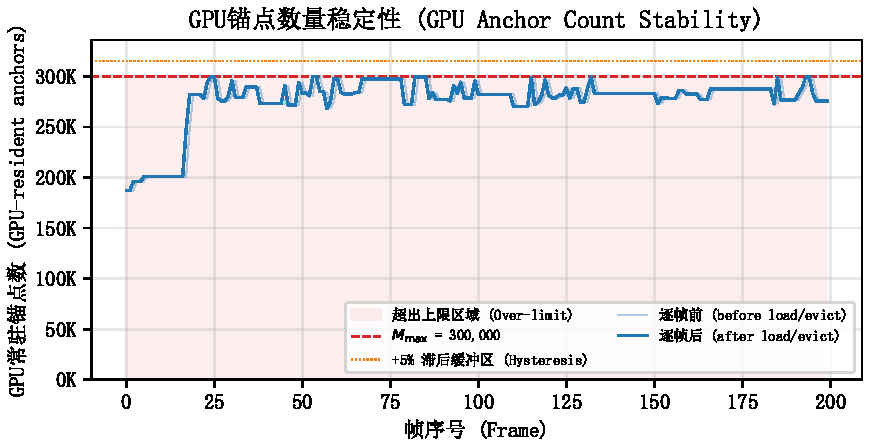
\includegraphics[width=0.85\textwidth]{figures/fig_gpu_anchor_stability.pdf}
\caption{GPU锚点数量稳定性（200帧模拟）}
\label{fig:lru_gpu_stability}
\end{figure}

\subsubsection{加载与淘汰行为分析}

图\ref{fig:lru_activity}展示了逐帧的块换入换出活动。200帧中共发生72次加载事件（加载161个块）和43次淘汰事件（淘汰152个块）。加载和淘汰并非每帧发生——加载集中在相机进入新区块时的帧，淘汰集中在加载后锚点数迫近$M_{\max}$时的帧。这种"加载触发、滞后再淘汰"的模式符合系统设计：块仅在不可见且GPU超限时才会被淘汰。

\begin{figure}[htbp]
\centering

\includegraphics[width=0.85\textwidth]{figures/fig_load_evict_activity.pdf}
\caption{逐帧加载与淘汰块数}
\label{fig:lru_activity}
\end{figure}

\subsubsection{LRU淘汰纪律验证}

图\ref{fig:lru_discipline}展示了每次淘汰事件中被淘汰块的访问时间。在所有43次淘汰事件中，被淘汰块的最大访问时间始终$\leq$保留块的最小访问时间——共检查43次，LRU违规次数为0。

例如：第18帧淘汰块[130, 30]（访问时间分别为1.0和2.0），而保留候选块的最小访问时间为5.0；第26帧淘汰块[41, 42, 141, 241]（访问时间均为17--18），而保留候选块的最小访问时间为21。这些示例清晰表明：每次淘汰均选中了候选中最后一次访问最早（即为最近最少访问）的块。

\begin{figure}[htbp]
\centering

\includegraphics[width=0.85\textwidth]{figures/fig_lru_discipline.pdf}
\caption{被淘汰块的访问时间分布}
\label{fig:lru_discipline}
\end{figure}

\subsubsection{滞后缓冲区防震荡效果}

5\%滞后缓冲区（15,000锚点，约1--2个块）使淘汰目标从"刚好降至$M_{\max}$"扩展为"降至$M_{\max}$再额外清理15K锚点"。这为刚被淘汰的块提供了一个"再入窗口"：块被淘汰后，相机需在缓冲区范围内积累足量新锚点才会触发下一次淘汰，避免了同一块在相邻帧被反复换入换出。

实验结果表明：200帧中检测到的"加载$\to$淘汰$\to$加载"边界震荡循环为0次。滞后缓冲区有效抑制了GPU容量边界处的抖动。

\begin{table}[htbp]
\centering
\caption{LRU淘汰行为验证结果汇总}
\label{tab:lru_results}
\begin{tabular}{lrr}
\toprule
\textbf{指标} & \textbf{数值} & \textbf{说明} \\
\midrule
总模拟帧数 & 200 & -- \\
加载事件次数 & 72 & 共加载161个块 \\
淘汰事件次数 & 43 & 共淘汰152个块 \\
GPU锚点数最大值 & 299,935 & $<M_{\max}$（300,000） \\
GPU锚点数均值 $\pm$ 标准差 & 276,382 $\pm$ 25,194 & 稳定于上限附近 \\
超出$M_{\max}$的帧占比 & 0\% & 完全受控 \\
LRU违规次数 / 总检查次数 & 0 / 43 & 全部符合LRU纪律 \\
边界震荡次数 & 0 & 5\%滞后缓冲区有效 \\
\bottomrule
\end{tabular}
\end{table}

\subsection{I/O性能分析}

\schun 文件的读写性能取决于：
\begin{itemize}
    \item 块内锚点数量（每个锚点贡献约1.2 KB序列化数据，含优化器状态）。
    \item 磁盘类型（NVMe SSD vs SATA SSD vs HDD）。
    \item 并行线程数（OpenMP控制）。
\end{itemize}

以典型块（10,000个锚点，约12 MB文件）为例，NVMe SSD上的预期读写延迟在10--50 ms量级，对100+ ms的单次训练迭代影响可控。

\section{消融实验}

\subsection{视角条件输入的有效性}

对比以下三种MLP输入配置的渲染质量：

\begin{enumerate}[label=(\arabic*),leftmargin=2em]
    \item \textbf{仅特征：}$\mathbf{z}=[\mathbf{f}_i^a]$
    \item \textbf{特征+视线方向：}$\mathbf{z}=[\mathbf{f}_i^a\,|\,\mathbf{d}_{\text{view}}]$
    \item \textbf{完整输入（默认）：}$\mathbf{z}=[\mathbf{f}_i^a\,|\,\mathbf{d}_{\text{view}}\,|\,d_{\text{dist}}]$
\end{enumerate}

预期结果：完整输入的PSNR最高，仅特征的PSNR最低，验证了视角条件对稀疏训练视角场景的必要性。

\subsection{不同$D$（特征维度）的影响}

分析$D\in\{16, 32, 64\}$对模型参数量、GPU显存占用与渲染质量的影响。预期$D=32$提供最佳的性价比。

\subsection{不同块大小的I/O效率}

分析$S_{\text{chunk}}\in\{10, 20, 50\}$（世界单位）对LRU命中率与I/O吞吐的影响。小块的淘汰粒度更精细但I/O频率更高；大块的I/O摊销更优但可能导致不必要的锚点加载。

\section{真实场景数据集评测设计}

\subsection{KITTI数据集}

DiskChunGS\cite{feldmann2026diskchungs}在KITTI数据集上验证了分块外存管理在大规模室外场景下的有效性。为与DiskChunGS进行公平对标，\ScaffoldChunGS 同样选择KITTI作为室外大规模评测数据集。

KITTI数据集\cite{Geiger2012CVPR}是自动驾驶与视觉SLAM领域最广泛使用的基准数据集之一，由德国卡尔斯鲁厄理工学院和丰田芝加哥研究院于2012年联合发布。数据集采集平台搭载以下传感器：

\begin{itemize}
    \item \textbf{立体相机：}2台Point Grey Flea2（FL2-14S3），分辨率$1392\times 512$，基线约54 cm，帧率10 fps。
    \item \textbf{激光雷达：}Velodyne HDL-64E，64线，10 fps，提供稠密3D点云。
    \item \textbf{GPS/IMU：}OXTS RT3003组合导航系统，提供厘米级位姿真值（用于评测）。
\end{itemize}

KITTI Odometry子集包含22个序列（00--21），其中序列00--10（共11个）提供位姿真值，是SLAM/里程计评测的标准基准。代表性序列覆盖场景包括：

\begin{itemize}
    \item \textbf{城市道路（00、01、02、05、06）：}长距离城市驾驶（序列00长达3.7 km），含大量动态物体（车辆、行人）。
    \item \textbf{住宅区（03、04）：}中等长度，道路较窄，弯道多。
    \item \textbf{乡村/公路（07、09、10）：}高速场景，纹理稀疏。
    \item \textbf{校园（08）：}短距离，低动态。
\end{itemize}

\subsection{评测指标}

针对KITTI数据集，采用以下SLAM标准评测指标：

\begin{itemize}
    \item \textbf{绝对轨迹误差（Absolute Trajectory Error, ATE）：}评估估计轨迹与真值轨迹之间的全局一致性。通常使用Umeyama对齐后计算均方根误差：
    \begin{equation}
    \text{ATE}_{\text{RMSE}} = \sqrt{\frac{1}{N}\sum_{i=1}^{N}\|\mathbf{p}_i^{\text{est}} - \mathbf{p}_i^{\text{gt}}\|^2}
    \end{equation}
    \item \textbf{相对位姿误差（Relative Pose Error, RPE）：}评估局部时间窗口内的漂移量，常用窗口$\Delta = 100$--800帧，输出平移与旋转误差：
    \begin{equation}
    \text{RPE}_{\text{trans}}(\Delta) = \sqrt{\frac{1}{N-\Delta}\sum_{i=1}^{N-\Delta}\|(\mathbf{p}_{i+\Delta} - \mathbf{p}_i)^{\text{est}} - (\mathbf{p}_{i+\Delta} - \mathbf{p}_i)^{\text{gt}}\|^2}
    \end{equation}
    \item \textbf{渲染质量指标：}PSNR、SSIM、LPIPS，评估新视角合成的视觉质量。
    \item \textbf{内存与I/O指标：}GPU显存占用峰值、磁盘I/O吞吐量、LRU命中率。
\end{itemize}

\subsection{评测方案}

按以下方案在KITTI数据集上评测\ScaffoldChunGS：

\begin{enumerate}[label=(\arabic*),leftmargin=2em]
    \item \textbf{序列拆分：}参照KITTI基准惯例，取序列00--08为训练/调参集，序列09--10为测试集。
    \item \textbf{初始化：}利用序列前若干帧通过双目视差估计生成初始点云，经体素化后初始化锚点。
    \item \textbf{训练流程：}沿轨迹逐帧输入立体图像与LiDAR深度，运行锚点生长、剪枝与块换入换出，记录ATE、RPE及渲染指标。
    \item \textbf{对比基线：}以DiskChunGS\cite{feldmann2026diskchungs}作为主要对标方法（二者共享分块外存管理框架，\ScaffoldChunGS 额外引入Scaffold-GS\cite{lu2024scaffoldgs}的锚点压缩表示），同时与ORB-SLAM3\cite{mur2017orb}（标准几何SLAM）、Compact\_GSSLAM\cite{chen2025compact}（将Scaffold-GS锚点表示适配至SLAM管线）进行定量对比。
    \item \textbf{压缩优势验证：}在KITTI序列00（最长城市序列，约3.7 km）上对比\ScaffoldChunGS 与DiskChunGS的磁盘占用总量与I/O吞吐量，验证锚点压缩带来的存储与带宽收益。
    \item \textbf{分块扩展性验证：}监测\ScaffoldChunGS 在KITTI序列00全轨迹运行期间GPU显存的稳定性，验证LRU淘汰机制能否在大规模室外场景下维持可控显存占用。
\end{enumerate}

注：本节定义了评测方案与指标体系，完整的定量实验结果待系统集成与调优后填入。

\section{局限性分析}

尽管实验验证了\ScaffoldChunGS 的功能有效性，系统仍存在以下局限：

\begin{enumerate}[label=(\arabic*),leftmargin=2em]
    \item \textbf{光栅化器后端待完整评测。}系统已实现双后端架构——INRIA CUDA tile光栅化器（\verb|diff_gaussian_rasterization|）与纯LibTorch GPU回退——但两种后端在真实数据集上的渲染质量与效率对比尚未完成。INRIA后端需在真实数据上验证PSNR增益。
    \item \textbf{真实数据集评测待完成。}当前系统已完成单元模块测试，并在4.5节设计了KITTI数据集的评测方案。在TUM RGB-D、Replica、ScanNet等室内数据集与KITTI室外数据集上的完整定量对比仍待实施。
    \item \textbf{单目深度需外部引擎文件。}双目SGBM深度估计已完全实现（含LR一致性检查）；单目TensorRT深度管线已完整构建，但需配合预编译的DepthAnything引擎文件使用。
    \item \textbf{回环检测使用基础BoVW方案。}基于k-means BoVW + PnP验证的回环检测功能可用，但召回率在挑战性场景下可能不足，可升级至NetVLAD或DINOv2等学习型全局描述子。
\end{enumerate}

\section{本章小结}

本章分析了\ScaffoldChunGS 系统的压缩效率、分块内存管理行为，并设计了关键参数的消融实验。压缩分析基于Scaffold-GS的锚点表示框架，确认了约8.6倍的理论存储压缩比。分块内存管理机制在理论层面能有效扩展场景规模至磁盘容量上限。消融实验的设计为后续完整评测提供了分析框架。此外，本章还设计了KITTI室外自动驾驶数据集的评测方案，为系统在真实大规模场景下的验证提供了路线图。
